\label{chap:design}

\epigraph{If you drive a car, it makes little difference what brand it is: all cars are driven
in essentially the same way. The same applies to computers. If you have a
Windows PC, the user interface won’t be affected by your computer hardware.
This is definitely not the case for industrial robots.}{\textit{Albert Nubiola \\ CEO at RoboDK}}

\par This chapter gets the reader acquainted with the RoboDK software. Firstly, the history and features of the RoboDK software are described. Secondly, the RoboDK robot library and RoboDK API are outlined. Finally, at the end of the chapter, a short introduction to RoboDK post processors is given. It is followed by  \hyperref[chap:implementation]{Chapter 4}, where the knowledge gained is used practically. 

\section{RoboDK overview}

RoboDK (short for robot development kit) is a development platform for industrial robotic arm offline and online programming and simulation. 
RoboDK (the company) was founded by Albert Nubiola and Lauren Ierullo in January 2015 as a spin-off company from the \href{https://en.etsmtl.ca/unites-de-recherche/coro/accueil?lang=en-CA}{CoRo laboratory}   at ETS University in Montreal, Canada. RoboDK is a commercial version of \href{https://www.parallemic.org/RoKiSim.html}{RoKiSim}, a multiplatform educational software tool for 3D simulation of serial 6-axis robotic arms \cite{robodkoverview}.

\subsection{RoboDK features}

The following section highlights some of the features RoboDK has to offer: 

\begin{itemize}
\item graphical user interface,
\item drag-and-drop functionality, 
\item support for 3D file formats -- importing objects and creating new tools using 3D files such as \mintinline{shell-session}{STL}, \mintinline{shell-session}{STEP} and \mintinline{shell-session}{IGES},
\item CAD-to-path features -- generating robot programs directly from curves placed on station objects 
\item external axes -- integrating external axes to extend the robotic arm’s reachability,
\item generating programs -- generating programs for various robotic arm manufacturers,
\item running programs on the fly –- executing programs directly from an external computer,
\item real-time monitoring –- viewing the robotic arm state on an external computer,
\item computer aided manufacturing for robotic arms -- converting 5-axis CNC toolpaths to robotic arm programs and using a robotic arm like a 5-axis CNC,
\item automated path solving -- avoiding robotic arm errors, including singularities, joint limits and collisions,
\item fast collision detection -- defining the object interactions, 
\item advanced use -- creating robotic arm programs from an external computer using a higher programming language. The RoboDK API is available in Python, C\#, Visual Basic, C++, and Matlab,
\item simulating 2D vision cameras -- testing image recognition algorithms in the simulation environment,
\item multiple robotic arms simulation -- synchronizing and programming multiple robotic arms and moving them at the same time, 
\item customizable post processors -- integrating specific sensors or actuators such as grippers, force control, image processing, etc. \cite{robodkfeatures}.
\end{itemize}

\subsection{RoboDK licence and versions}

RoboDK offers free (limited), educational or professional versions. 
The software is available for Windows, MacOS, Ubuntu Linux, Android or iOS. It supports either 32-bit or 64-bit versions of the abovementioned operating systems. At the time of writing this document, the latest version of RoboDK is 5.2. The complete RoboDK revision history is available \href{https://robodk.com/whatsnew}{online} \cite{robodkversions}. 

\section{RoboDK robot library}

RoboDK supports offline programming and has an extensive robotic arm library supporting robotic arm controllers from various manufacturers, including, but not limited to:

\begin{itemize}
    \item ABB, 
    \item FANUC, 
    \item KUKA ,
    \item Motoman, 
    \item Universal Robots.
\end{itemize}
Models of industrial robotic arms in RoboDK have the same properties as if used with an physical robotic arm controller. The RoboDK library can be accessed \href{https://robodk.com/library}{online} either via a browser or in the RoboDK application itself (keyboard shortcut \mintinline{shell-session}{Ctrl+Shift+O}) \cite{robodklibrary}.


\section{RoboDK interface}

The interface of RoboDK consists of the main menu, the toolbar, the station tree, the status bar, the 3D view, and the robot panel. A picture of the RoboDK interface is shown in Figure \ref{fig:robodkinterface}. An extensive documentation for RoboDK is available \href{https://robodk.com/doc/en/Basic-Guide.html#Start}{online} \cite{robodkinterface}.

\subsection{RoboDK station}

A RoboDK project containing a robotic arm, robotic arm tools, additional CAD files, robotic arm frames, and a robotic arm program is called a station. A RoboDK station is saved as one file (\mintinline{shell-session}{.rdk} extension).  The FANUC M-20iA/35M model from the RoboDK robotic arm library is used in this study because it is readily available in the RoboDK library and differs from the FANUC M-20iA/20M robotic arm used in the LSP station at HiLASE only in payload capacity. Robot files in RoboDK have a \mintinline{shell-session}{.robot} extension \cite{robodkstation}.

\begin{figure}[h]
    \centering
    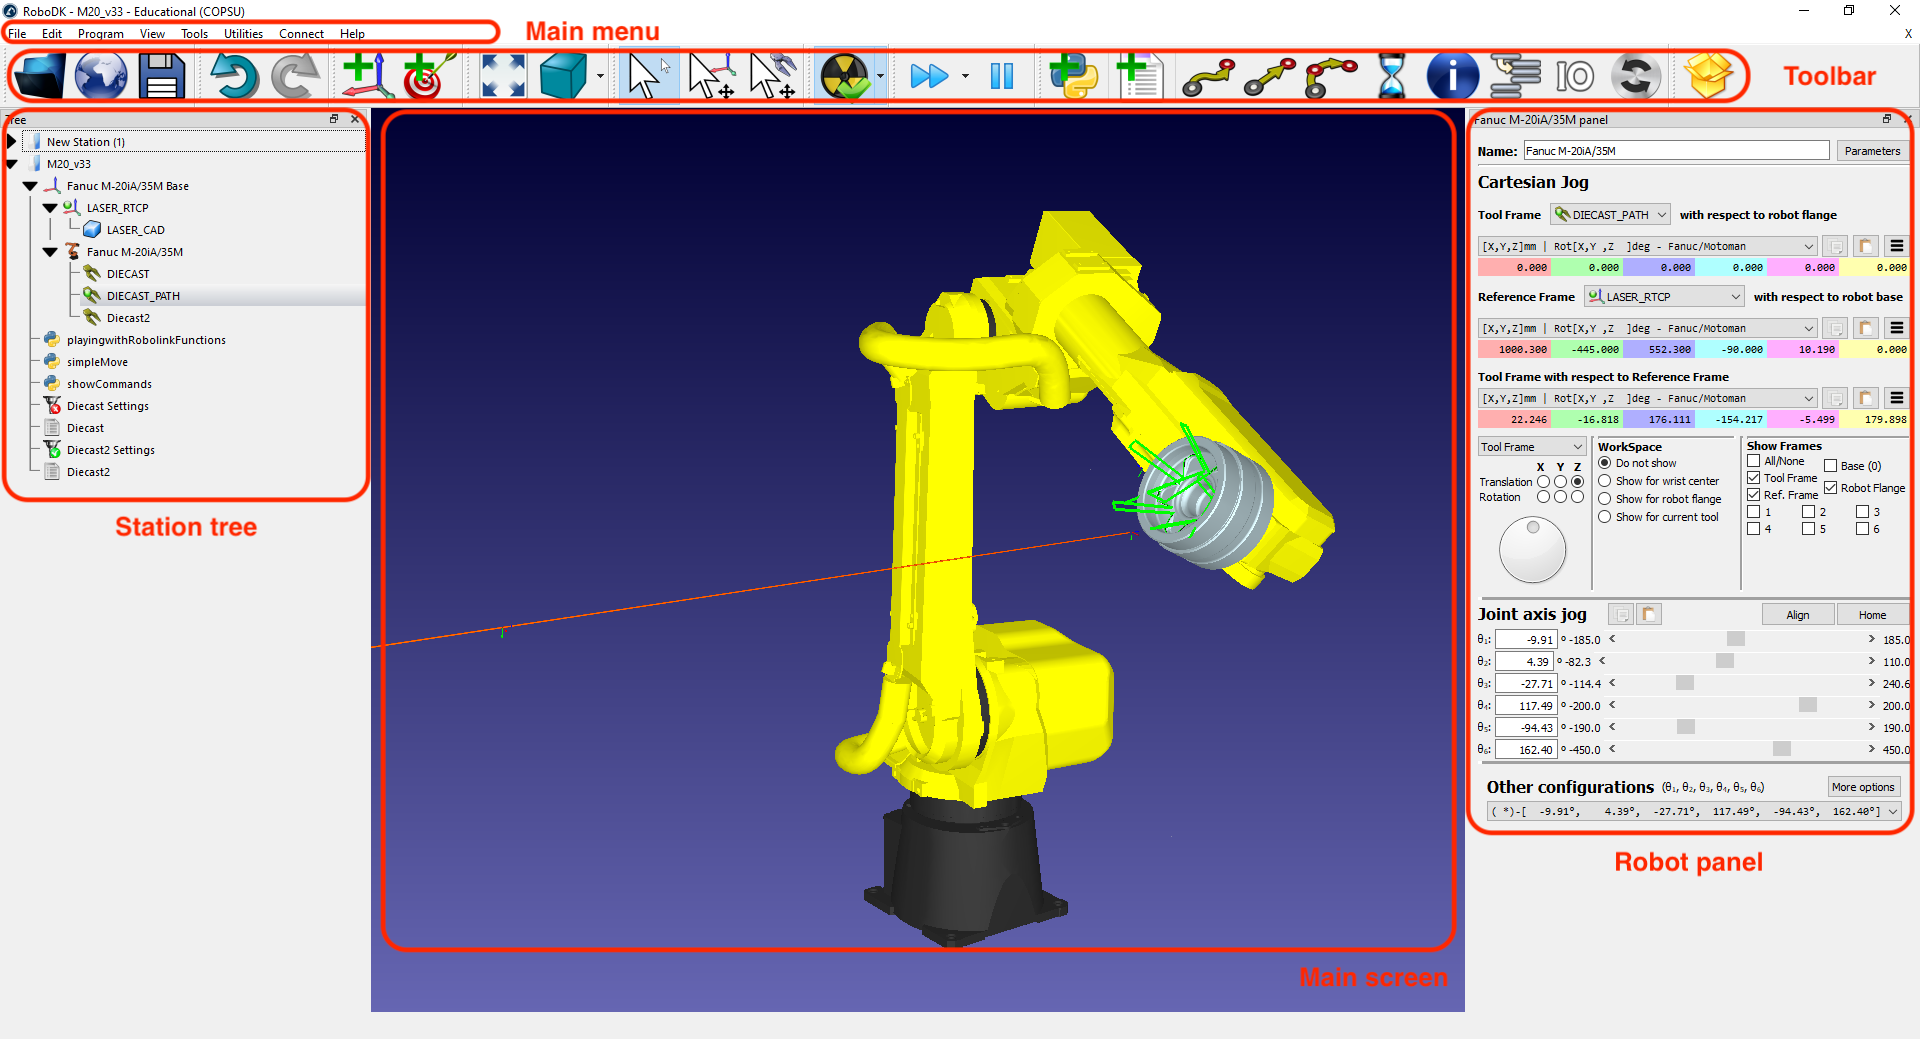
\includegraphics[width=0.9\linewidth]{img/robodk_interface_v_2.png}
    \caption{RoboDK version 5.2 running on Windows 10}
    \label{fig:robodkinterface}
\end{figure}

\section{RoboDK API}

RoboDK provides a graphical user interface (GUI) to simulate and program industrial robotic arms. No programming experience is required to simulate and program robotic arms using the GUI. Unfortunately, the GUI has some limitations when used for simulation and offline programming. If such a situation arises, then the RoboDK application interface (API) can be used to extend the capabilities of RoboDK.

The API provides a set of routines and commands to RoboDK, enabling the user to program the robotic arm using high-level programming languages. The RoboDK API is implemented in Python, C\#, C++, Visual Basic (.NET) and Matlab. Any of these programming languages can be used to simulate and program any robotic arm. The API can conveniently handle the following tasks:

\begin{itemize}
    \item automating simulation,
    \item offline programming,
    \item online programming.

\end{itemize}

The RoboDK API for Python consists of the following modules:


\begin{itemize}
    \item \mintinline{text}{robolink} module, 
    \item \mintinline{text}{item} module, 
    \item \mintinline{text}{robodk} module.
\end{itemize}

The RoboDK API is described in more detail in \hyperref[chap:implementation]{Chapter 4}.

\section{RoboDK Add-ins}

\subsection{RoboDK Add-in interface}

Add-ins extend RoboDK's functionality. Add-ins can be developed by using the RoboDK Add-in interface. The RoboDK Add-in interface is linked natively to the core of RoboDK \cite{robodkaddininterface}.

\subsection{RoboDK Add-in for SolidWorks}

Solidworks is a professional 3D CAD modelling application. The RoboDK Add-in for SolidWorks allows to combine SolidWorks' 3D CAD modelling features with robotic arm simulation and offline programming in RoboDK and considerably simplifies the programmer's workflow. The programmer can load the 3D models created in SolidWorks directly to RoboDK. Groups of curves or points can also be loaded to RoboDK, and robotic arm programs can be generated from the curves or points subsequently.

\subsubsection*{SolidWorks RoboDK Add-in toolbar}

The RoboDK Add-in for SolidWorks is accessible directly from the SolidWorks toolbar.  The RoboDK Add-in toolbar is shown in Figure  \ref{fig:solidworkstoolbar}. The Add-in toolbar presents the programmer with several functionalities:

\begin{itemize}
    \item \mintinline{shell-session}{AutoSetup} -- the user selects the geometry (curves and points) and the model, the curves are automatically transferred to RoboDK,
    \item \mintinline{shell-session}{LoadPart} -- only loads the 3D model from SolidWorks to RoboDK without importing the curves or points,
    \item \mintinline{shell-session}{LoadPoints} -- loads points to RoboDK as a new object. Selected surfaces are used to calculate the curve normals, 
    \item \mintinline{shell-session}{LoadCurves} --  loads curves selected in RoboDK as a new object. Selected surfaces are used to calculate curve normals, 
    \item \mintinline{shell-session}{Settings} -- opens default settings window \cite{robodksolidworks}.
\end{itemize}

\begin{figure}[h]
    \centering
    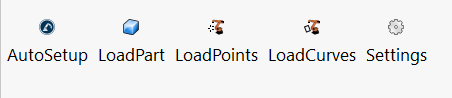
\includegraphics[width=0.6\linewidth]{img/solidworks_toolbar.PNG}
    \caption{SolidWorks RoboDK Add-in toolbar}
    \label{fig:solidworkstoolbar}
\end{figure}


%%%%%% TO MUCH USELESS INFORMATION, WILL BE LEFT OUT FOR NOW %%%% 

\begin{comment}

\subsubsection*{Importing curves from Solidworks}

To import curves from SolidWorks to RoboDK, SolidWorks offers two options:

\begin{enumerate}

\item PŘEDĚLAT FORMU, ABY BYLO PODOBNÉ.

\item \textbf{Opening an existing RoboDK station} - Using the \mintinline{shell-session}{Settings} control element of the SolidWorks RoboDK Add-in and then selecting the current project with the \mintinline{shell-session}{Load Project...} button. The next step is to click the \mintinline{shell-session}{LoadCurves} button and highlight the curves that define the robotic arm path and the adjacent surfaces of these curves. Lastly, the action is confirmed by pressing the \mintinline{shell-session}{checkmark} button. The curve is then opened in the selected project. 

\item \textbf{Creating a new RoboDK station} - In this case, the robot path is selected the same way as described in the previous point. A new RoboDK station containing the robotic arm path is opened after pressing the \mintinline{shell-session}{checkmark} button.

\end{enumerate}

\end{comment}


\section{RoboDK post processors}

Post processors generate robot programs for robotic arm controllers from robotic arm simulations. Post processors are essential for offline programming of robotic arms. A post processor defines the vendor-specific rules a robotic arm program must follow. A robotic arm must be linked to a post processor in RoboDK to be able to generate a robotic arm controller program. The post processors available in RoboDK by default can be found \href{https://robodk.com/doc/en/Post-Processors.html#AvailablePosts}{online}.  
A post processor in RoboDK is a Python script (\mintinline{shell-session}{.py} extension). All the post processors of RoboDK are located in the
\mintinline{shell-session}{C:/RoboDK/Posts/} folder (in case of the Windows operating system).  To use a post processor it must be placed in the \mintinline{shell-session}{C:/RoboDK/Posts/} folder. The user can modify an existing post processor or create a new one from scratch. Modifications of post processors are described in \hyperref[chap:implementation]{Chapter 4} in more detail \cite{robodkposts}. 